% Figure 1a: how each retrained agent gets its goal-suit belief.
% Build: tectonic arms.tex  (standalone, about 3.3 x 2.4 in)
\documentclass[tikz,border=1pt]{standalone}
\usepackage[T1]{fontenc}
\usepackage[scaled=0.95]{helvet}
\renewcommand{\familydefault}{\sfdefault}
\usepackage{pifont}
\usetikzlibrary{positioning,arrows.meta,calc}

% Okabe-Ito, the same colours as the bars in teaser.pdf
\definecolor{blue}{HTML}{0072B2}
\definecolor{verm}{HTML}{D55E00}
\definecolor{sky}{HTML}{56B4E9}
\definecolor{grey}{HTML}{666666}
\definecolor{ink}{HTML}{222222}

\begin{document}
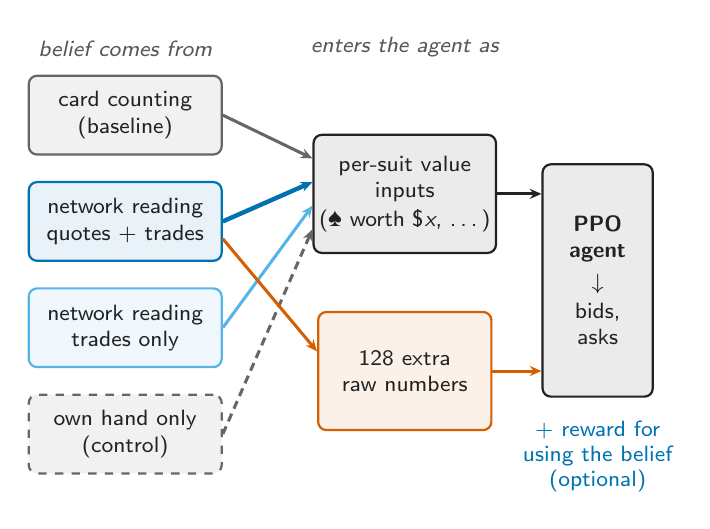
\begin{tikzpicture}[
    font=\fontsize{8.5}{9.5}\selectfont,
    >={Stealth[length=4.2pt,width=3.6pt]},
    box/.style={draw=#1, fill=#1!9, rounded corners=3pt, line width=0.8pt,
                align=center, inner sep=2pt, text=ink},
    src/.style={box=#1, minimum width=2.45cm, minimum height=1.0cm},
    mid/.style={box=#1, minimum width=2.2cm, minimum height=1.5cm},
    head/.style={font=\fontsize{8.5}{9.5}\selectfont\itshape, text=grey!85!black},
    flow/.style={->, line width=1.1pt, draw=#1, rounded corners=4pt},
  ]
  % ---------- left column: where the belief comes from
  \node[src=grey]  (cc)   at (0, 0)     {card counting\\(baseline)};
  \node[src=blue]  (qt)   at (0,-1.35)  {network reading\\quotes + trades};
  \node[src=sky]   (tr)   at (0,-2.70)  {network reading\\trades only};
  \node[src=grey, dashed] (hand) at (0,-4.05) {own hand only\\(control)};
  \node[head, above=3pt of cc] {belief comes from};

  % ---------- middle column: how it enters the agent
  \node[mid=ink]  (psv) at (3.55,-1.0) {per-suit value\\inputs\\[1pt]{\footnotesize(\ding{171} worth \$\textit{x}, \ldots)}};
  \node[mid=verm] (raw) at (3.55,-3.25) {128 extra\\raw numbers};
  \node[head] at (psv |- cc.north) [anchor=south, yshift=3pt] {enters the agent as};

  % ---------- right: the agent
  \node[box=ink, minimum width=1.4cm, minimum height=2.95cm] (ppo) at (6.0,-2.1)
       {\textbf{PPO}\\\textbf{agent}\\[2pt]$\downarrow$\\[1pt]bids,\\asks};
  \node[text=blue, align=center, below=5pt of ppo, font=\fontsize{8}{9}\selectfont]
       {+ reward for\\using the belief\\(optional)};

  % ---------- paths into the per-suit value inputs (fanned along its west side)
  \coordinate (in1) at ($(psv.west)+(0, 0.45)$);
  \coordinate (in2) at ($(psv.west)+(0, 0.15)$);
  \coordinate (in3) at ($(psv.west)+(0,-0.15)$);
  \coordinate (in4) at ($(psv.west)+(0,-0.45)$);
  \draw[flow=grey]               (cc.east)   -- (in1);
  \draw[flow=blue, line width=1.6pt] (qt.east) -- (in2);
  \draw[flow=sky]                (tr.east)   -- (in3);
  \draw[flow=grey, dash pattern=on 3pt off 2pt] (hand.east) -- (in4);
  % quotes + trades also feeds the raw features
  \draw[flow=verm] ($(qt.east)+(0,-0.22)$) -- ($(raw.west)+(0,0.25)$);

  % ---------- both inputs go to the agent
  \draw[flow=ink]  (psv.east) -- (psv.east -| ppo.west);
  \draw[flow=verm] (raw.east) -- (raw.east -| ppo.west);
\end{tikzpicture}
\end{document}
